\paragraph{Aufbau}
Der Aufbau gleicht weitestgehend dem Aufbau der historischen Rutherfordstruung (Abbildung \ref{fig:aufbau}).
Eine $^{241}\symup{Am}$-Quelle befindet sich in einer evakuierbaren Kammer.
Der Träger für die Folien kann in den Strahlengang der Quelle gefahren werden.
Der Detektor ist schwenkbar auf einer Goniometerscheibe montiert und ermöglicht das Messen der Zählraten in Abhängigkeit vom Winkel.
Es liegt ein Oberflächensperrschichtzähler als Detektor vor.
Das Zählwerk ist mit dem Detektor verbunden und kann mit einem Zeitgeber verwendet werden.
Die entstehenden Pulse können auch mit einem Oszilloskop abgebildet werden.
Für die Evakuierung steht eine Drehschieberpumpe zur Verfügung.
Hiermit können Drücke bis ca. $\SI{80}{\milli bar}$ erreicht werden.
Zur Abschirmung der äußeren Streustrahlung gibt es einen Deckel, mit dem die Apparatur abgedunkelt werden kann.

\begin{figure}[h!]
  \centering
  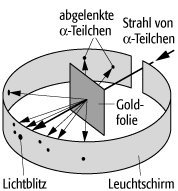
\includegraphics[width=5cm]{images/aufbau_rutherfordstreuung.jpg}
  \caption{Aufbau der historischen Rutherford-Streuung, modifiziert \cite{aufbau}}
  \label{fig:aufbau}
\end{figure}

\FloatBarrier

\paragraph{Durchführung}
Für eine maximale Unsicherheit von ca. $\SI{3}{\%}$ wird eine Mindestzählrate von  $N=1000$ angestrebt.
\\Zunächst wird der Detektor gerade auf die Quelle ausgerichtet.
Dann wird zur Bestimmung der $\texttt{Foliendicke}$ die Pulshöhe $U$ in V am Oszilloskop in Abhängigkeit des Kammerdrucks $p$ gemessen.
Dabei wird die Kammer evakuiert und nach und nach wird das Ventil geöffnet.
Die Messung wird einmal ohne Folie und einmal mit Folie im Strahlengang durchgeführt, um auf den Energieverlust durch die Folie schließen zu können.
\\Zur Messung des $\texttt{Differenziellen Wirkungsquerschnitts}$ $\displaystyle{ \frac{d\sigma (\vartheta)}{d\Omega}}$ wird die Folie in den Strahlengang gebracht.
Der Detektor wird in Schritten von $\SI{0.1}{°} - \SI{0.5}{°}$ um das Streuzentrum gedreht.
Als Messdaten werden die Aktivität $A$ und der Winkel $\vartheta$ notiert.
\\Den Effekt der $\texttt{Mehrfachstreuung}$ in den Folien wird mit einer Messung verschiedener Foliendicken untersucht.
Hierfür werden bei $\vartheta = \SI{-1}{°}$ zwei Goldfolien mit angegebenen Dicken von $d=\SI{2}{\micro m}$ und $d = \SI{4}{\micro m}$ verwendet.
\\Abschließend wird der Zusammenhang der Aktivität $A$ und der $\texttt{Ordnungszahl}$ $Z$ betrachtet.
Für drei Folien verschiedener Materialien werden bei einem Winkel von $\vartheta = \SI{4.2}{°}$ die Aktivitäten gemessen.
Die verwendeten Folien sind:
\begin{itemize}
	\item Aluminium: $d=\SI{3}{\micro m}$
	\item Bismut: $d=\SI{2}{\micro m}$
	\item Gold: $d=\SI{4}{\micro m}$.
\end{itemize}
%Aufbau
%- Quelle
%- Folie
%- Detektor, Winkelverstellbar
%- Vakuumpumpe
%- Zähler mit Taktung (Zeit einstellbar)
%
%Durchführung, Messung der:
%- Dicke der Folie mit Bethe-Bloch (einmal mit Folie, einmal ohne Folie, in Abhängigkeit des Drucks)
%- Winkelabhängigkeit der Rutherfordstreuung einer Folie
%- Z-Abhängigkeit mit verschiedenen Folien
%- große Winkel?
%
